\documentclass[11pt,]{article}
\usepackage{lmodern}
\usepackage{amssymb,amsmath}
\usepackage{ifxetex,ifluatex}
\usepackage{fixltx2e} % provides \textsubscript
\ifnum 0\ifxetex 1\fi\ifluatex 1\fi=0 % if pdftex
  \usepackage[T1]{fontenc}
  \usepackage[utf8]{inputenc}
\else % if luatex or xelatex
  \ifxetex
    \usepackage{mathspec}
  \else
    \usepackage{fontspec}
  \fi
  \defaultfontfeatures{Ligatures=TeX,Scale=MatchLowercase}
\fi
% use upquote if available, for straight quotes in verbatim environments
\IfFileExists{upquote.sty}{\usepackage{upquote}}{}
% use microtype if available
\IfFileExists{microtype.sty}{%
\usepackage{microtype}
\UseMicrotypeSet[protrusion]{basicmath} % disable protrusion for tt fonts
}{}
\usepackage[margin=1in]{geometry}
\usepackage{hyperref}
\hypersetup{unicode=true,
            pdftitle={Displacement of fishing effort by Large Scale Marine Protected Areas},
            pdfborder={0 0 0},
            breaklinks=true}
\urlstyle{same}  % don't use monospace font for urls
\usepackage{natbib}
\bibliographystyle{chicago}
\usepackage{longtable,booktabs}
\usepackage{graphicx,grffile}
\makeatletter
\def\maxwidth{\ifdim\Gin@nat@width>\linewidth\linewidth\else\Gin@nat@width\fi}
\def\maxheight{\ifdim\Gin@nat@height>\textheight\textheight\else\Gin@nat@height\fi}
\makeatother
% Scale images if necessary, so that they will not overflow the page
% margins by default, and it is still possible to overwrite the defaults
% using explicit options in \includegraphics[width, height, ...]{}
\setkeys{Gin}{width=\maxwidth,height=\maxheight,keepaspectratio}
\IfFileExists{parskip.sty}{%
\usepackage{parskip}
}{% else
\setlength{\parindent}{0pt}
\setlength{\parskip}{6pt plus 2pt minus 1pt}
}
\setlength{\emergencystretch}{3em}  % prevent overfull lines
\providecommand{\tightlist}{%
  \setlength{\itemsep}{0pt}\setlength{\parskip}{0pt}}
\setcounter{secnumdepth}{5}
% Redefines (sub)paragraphs to behave more like sections
\ifx\paragraph\undefined\else
\let\oldparagraph\paragraph
\renewcommand{\paragraph}[1]{\oldparagraph{#1}\mbox{}}
\fi
\ifx\subparagraph\undefined\else
\let\oldsubparagraph\subparagraph
\renewcommand{\subparagraph}[1]{\oldsubparagraph{#1}\mbox{}}
\fi

%%% Use protect on footnotes to avoid problems with footnotes in titles
\let\rmarkdownfootnote\footnote%
\def\footnote{\protect\rmarkdownfootnote}

%%% Change title format to be more compact
\usepackage{titling}

% Create subtitle command for use in maketitle
\newcommand{\subtitle}[1]{
  \posttitle{
    \begin{center}\large#1\end{center}
    }
}

\setlength{\droptitle}{-2em}

  \title{Displacement of fishing effort by Large Scale Marine Protected
Areas\footnote{Work in progress, do not circulate}}
    \pretitle{\vspace{\droptitle}\centering\huge}
  \posttitle{\par}
  \subtitle{Updated on 2018-10-19}
  \author{Juan Carlos Villaseñor-Derbez\textsuperscript{1} John
Lynham\textsuperscript{2}}
    \preauthor{\centering\large\emph}
  \postauthor{\par}
      \predate{\centering\large\emph}
  \postdate{\par}
    \date{\textsuperscript{1}Bren School of Environmental Science and Management,
University of California Santa Barbara, Santa Barbara,
CA\newline \textsuperscript{2}Department of Economics, University of
Hawaii at Manoa, Honolulu, HI}

\usepackage{float}
\floatplacement{figure}{H}
\usepackage{lineno}
\linenumbers
\usepackage[bottom]{footmisc}
\usepackage{pdflscape}
\newcommand{\beginsupplement}{\setcounter{table}{0}  \renewcommand{\thetable}{S\arabic{table}} \setcounter{figure}{0} \renewcommand{\thefigure}{S\arabic{figure}}}

\begin{document}
\maketitle
\begin{abstract}
Large-scale Marine Protected Areas (LSMPAs) have seen a significant
increase over the last years. Fishing effort is effectively eliminated
within these protected areas upon implementation. The benefits of
reducing effort have been largely studied, and include increases in
abundance, biomass, and diversity within the bounded regions. These
no-take zones may produce spillover effects, which provide fish for
outside areas. However, the economic and ecological implications of
displacing fishing effort are not yet fully understood. Novel data
products that track fishing effort at the vessel-level allow us to
identify changes in fleet- and vessel-level behavior upon the
implementation of protected areas, as well as how these redistribute.
This papers evaluates the implications of implementing LSMPA, by
evaluating changes in fishing hours, showing that vessels in the
effected region reduce fishing effort after the implementation of PIPA.
Our results are robust to a set of specifications. We also track the
relative spatial allocation of fishing events thorugh time, and identify
that areas closer to PIPA show an increase in relative fishing hourse
due to the displacement of PIPA-fishing vessels. Our results not only
provide an impact evaluation of the effect of LSMPAs on fishing
activity, but provide insights into vessel redistribution dynamics,
which may have ecological and economic implications.
\end{abstract}

\clearpage

\hypertarget{introduction}{%
\section{Introduction}\label{introduction}}

Marine Protected Areas (MPAs) are intended to safeguard parts of the
ocean from fishing and other extractive activities. Current
international goals aim to protect 10\% of the ocean environments by
2020. In an effort to meet this target, the world has seen a rapid
increase in MPA coverage \citep{wood_2008,sala_2018}, largely driven by
a small number of Large Scale Marine Protected Areas (LSMPA)
\citet{singleton_2014,boonzaier_2016,alger_2017}). Due to weak property
rights, limited habitat transformation, and potentially lower management
costs, LSMPAs provide an opportunity to safeguard the oceans
\citet{game_2009}. Today, a small number of LSMPAs make up at least 80\%
of the managed areas in the ocean \citet{toonen_2013}. LSMPAs may be
instrumental in helping us achieve the 10\% target by 2020
\citep{mccauley_2016}.

Given the relatively recent establishment of most LSMPAs, very little is
known about their human dimensions and implication for fisheries
\citep{gray_2017}. As with customary MPAs, it is important that we
understand the socioeconomic implications of management interventions.
One issue of particular importance is that of the displacement or
redistribution of fishing effort, which may influence the outcomes of an
MPA \citep{smith_2003}. Theoretical models make different assumptions
about the way in which fishers will reallocate fishing effort after an
area closure. The few empirical works focus on small-scale fisheries and
rarely incorporate spatially explicit data. Despite these efforts,
marine conservation is yet to identify the response in fishing effort
and its management implications.

Recent advances in satellite tracking technologies and near real-time
identification of fishing activity provide us with an opportunity to
tackle increase governance and answer long-lasting questions. Here, we
ask, how do fishers respond to the implementation of LSMPA? After a
closure, and if they continue to fish, where do they reallocate fishing
effort? We use identification of fishing activity via Automatic
Identification Systems (AIS) and causal inference techniques to describe
the behavioral changes and spatial redistribution of the industrial tuna
purse seine fleet due to the implementation of a Large Scale Marine
Protected Areas in the Pacific Ocean.

Our work is novel in the sense that it provides empirical evidence of
the effect of Large Scale Marine Protected Areas in fishing behavior and
distribution and can help guide future interventions as countries march
towards meeting the targeted 10\% of ocean protection. Understanding how
effort is displaced from LSMPAs might provide insights into how the
industrial fleet would react to a high seas closure.

The paper is outlined as follows: Section \ref{background} provides more
information on Large Scale Marine Protected Areas and background on
empirical studies of effort redistribution. An overview of the Nauru
Agreement and associated countries, a description of the fleet that
operates in the region, and a brief history of PIPA is also included.
Section \ref{methods} describes our data and identification strategy.
Section \ref{results} presents our results, section \ref{discussion}
provides an extension of our results to other
LSMPAs\footnote{Not yet. but I think this would be interesting} and
discusses our
results\footnote{I might also include a section, after the background, where I explain the different theoretical models of effort redistribution and behavioral responses}.

\hypertarget{background}{%
\section{Background}\label{background}}

\hypertarget{large-scale-marine-protected-areas}{%
\subsection{Large Scale Marine Protected
Areas}\label{large-scale-marine-protected-areas}}

The cutoff at which an MPA is considered to be a LSMPA ranges from areas
larger than 30,000 km\textsuperscript{2} as defined by
\citet{desanto_2013} or areas larger than 250,000 km\textsuperscript{2},
as defined by \citep{toonen_2013}. Figure \ref{fig:LSMPAs_map} shows
LSMPAs that meet the later, and that are fully no take. LSMPAs are often
implemented in the pelagic environment, where the dominant human
activity is industrial fishing \citep{gray_2017,kroodsma_2018}. The
early literature on LSMPAs focused on the inherent challenges and
difficulties that come with a pelagic environment. \citet{kaplan_2010}
claimed that very large MPAs would result in excessive opportunity costs
and that these would be difficult to enforce. \citet{game_2009}
suggested that most of the challenges could be overcome with the
incorporation of technology, in what then became known as Dynamic Ocean
Management \citep{maxwell_2015}. The effectiveness and difficulties of
implementating LSMPAs are not the focus of this paper
\footnote{But see \citet{singleton_2014}, who provide an objective discussion of pros and cons of LSMPAs.}.
Instead, we focus on the effect and implications of the ones that
\emph{have been} implemented.

\begin{figure}
\centering
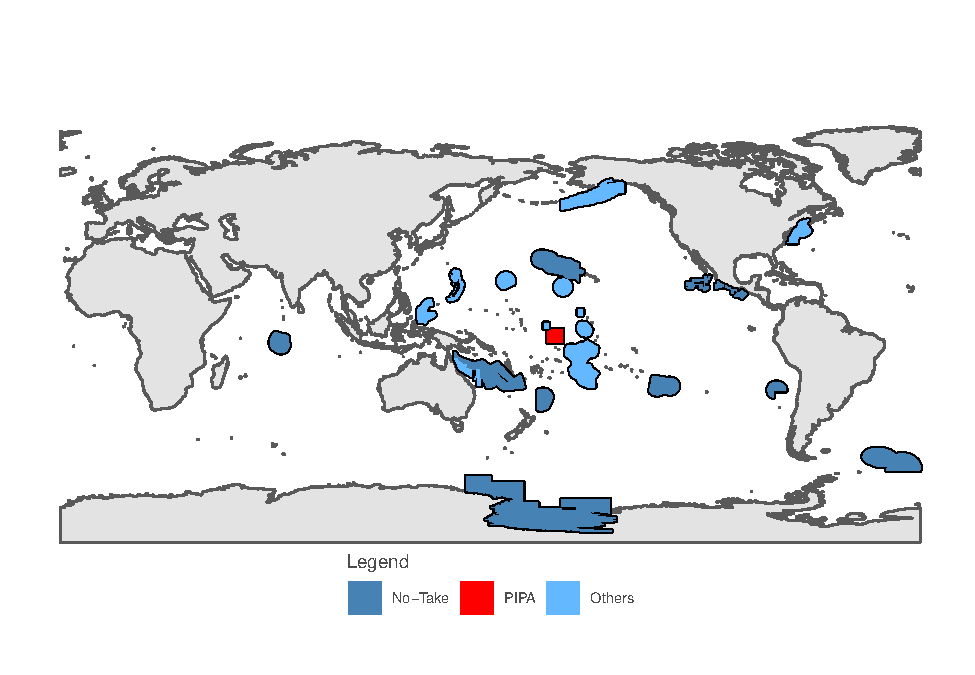
\includegraphics{C:/Users/JC/Documents/GitHub/MPA_displacement/docs/Manuscript_files/figure-latex/unnamed-chunk-2-1.pdf}
\caption{\label{fig:unnamed-chunk-2}\label{fig:LSMPAs_map}Large Scale Marine
Protected Areas. The map shows all areas larger than 250,000
Km\textsuperscript{2}. Areas in dark blue meet at least one of these
conditions: reported no take area is greater than 0, are categorized as
IUCN Ia or Ib, their designated english name is `Protected Area'.}
\end{figure}

LSMPAs were erroneously assumed to have little social implications due
to their remoteness. However, there have been calls to incorporate the
human dimensions into LSMPAs management and evaluation
\citep{agardy_2011,gray_2017}. Most research incorporating these
dimensions has focused on governance and enforcement of LSMPAs
(\emph{i.e.} \citet{alger_2017,christie_2017}), but they are yet to be
the focus of economic analyses \citep{gray_2017}. Overall, there has
been little empirical work regarding LSMPAs. Recent technological
advances in vessel-detection systems allows for the discovery and
advancement of many important facets of LSMPAs. For example,
\citep{mcdermott_2018} show that the anticipation of a LSMPA can lead to
preemptive overfishing, which can erode or delay the expected benefits
of the intervention. \citet{white_2017} combine shark tags and
vessel-tracking data to demonstrate that the fairly large Palmyra Atoll
National Wildlife Refuge (54,000 Km\textsuperscript{2}) protectes two
thrids of the tagged grey reef sharks by effectively excluding fishing
effort. More recently, \citep{bradley_2018} use similar data to
highlight cases of potential illegal shark fishing \emph{inside} a 2
million km\textsuperscript{2} shark sanctuary. To date, no studies have
evaluated the displacement of fishing effort due to LSMPA
implementation.

Spatial closures of this magnitude are likely to induce changes in
fishers' behavior. Theoretical models of fishing effort redistribution
range from the simplistic assumption that effort inside the bounded
region disappears, to spatially explicit models that reallocate fishing
effort based on habitat characteristics, presence of other vessels, and
expected returns \citep{smith_2003,hilborn_2006}. However, these focus
on the long term optimal equilibrium, and redistribution of fishing
effort may not always be optimal, especially over the first years
\citep{stevenson_2013}.

The empirical research that has been done in custumary sized MPAs
suggest that resource users may show idiosyncratic responses. For
example, \citet{stevenson_2013} show that a network of MPAs displaced
fishing effort farther away from ports, resulting in higher
\emph{perceived} costs, and increases in catch per unit effort.
\citet{cabral_2017} analyse the redistribution of fishing and
non-fishing vessels following the implementation of a network of MPAs in
California, and find that commercial dive boats follow a
fishing-the-line pattern, while some fishing boats follow an ideal free
distribution. More recently \citet{elahi_2018} used satellite tracking
data to show that a temporal spatial closure caused trawlers to maintain
effort but apply it more intensively elsewhere, particularly along the
borders and closer to shore. The way in which fishers react to a spatial
closure can have major implications in its outcome
\citep{smith_2003,hilborn_2006} highlighting the need to understand how
fishers react to the implementation of LSMPAs, and fishing effort
changes and is spatially redistributed. However, all these closures took
place within Exlcusive Economic Zones, where other regulations exist.
This may not always be the case for LSMPAs, where often the entire EEZ
is converted into a LSMPA, leaving fishers with the options of moving to
the high seas or other countries' EEZs.

\hypertarget{nauru-agreement-and-the-phoenix-island-protected-area}{%
\subsection{Nauru agreement and the Phoenix Island Protected
Area}\label{nauru-agreement-and-the-phoenix-island-protected-area}}

The Nauru Agreement was established in 1982 by a select group of Pacific
island nations to manage their important tuna resources. PNA Members
include Federated States of Micronesia, Kiribati, Marshall Islands,
Nauru, Palau, Papua New Guinea, Solomon Islands, and Tuvalu. The Nauru
Agreement regulated access of foreign vessels (\emph{i.e.} those from
non-PNA countries). Holding \textasciitilde{}80\% of the historical
purse seining grounds within their Exclusive Economic Zones, PNA
countries gained bargaining power when providing access to foreign
fleets \citep{havice_2010}.

The cooperation that emerged thanks to the PNA allowed for subsequent
agreements that strengthened fisheries management, like the Palau
Agreement, which limited the number of purse seiners at 205 vessels from
1995-2007\footnote{See \citet{havice_2010} for a detailed description of
  the Nauru, Palau, and Federal States of Micronesia agreements, their
  objectives, and outcomes.}. However, the most notable regulation is
their approach to manage fishing effort: a Vessel Day Scheme (VDS)
implemented in 2007 \citep{havice_2013}. This effectively modified how
fishing effort was managed, from number of vessels under the Palau
Agreement to fishing hours. The VDS works as follows: Each year,
scientific advisors recomend a total number of fishing vessel-days per
year. Hours are allocated to each PNA country based on catch history,
and they then use or sell fishing rights to other non-PNA countries
\citep{aqorau_2018}. While the effectiveness of this scheme has been
debated in terms of meeting their fishery management and conservation
objectives, the licensing significantly contributes to the economy of
these island nations \citep{havice_2010}.

\begin{figure}
\centering
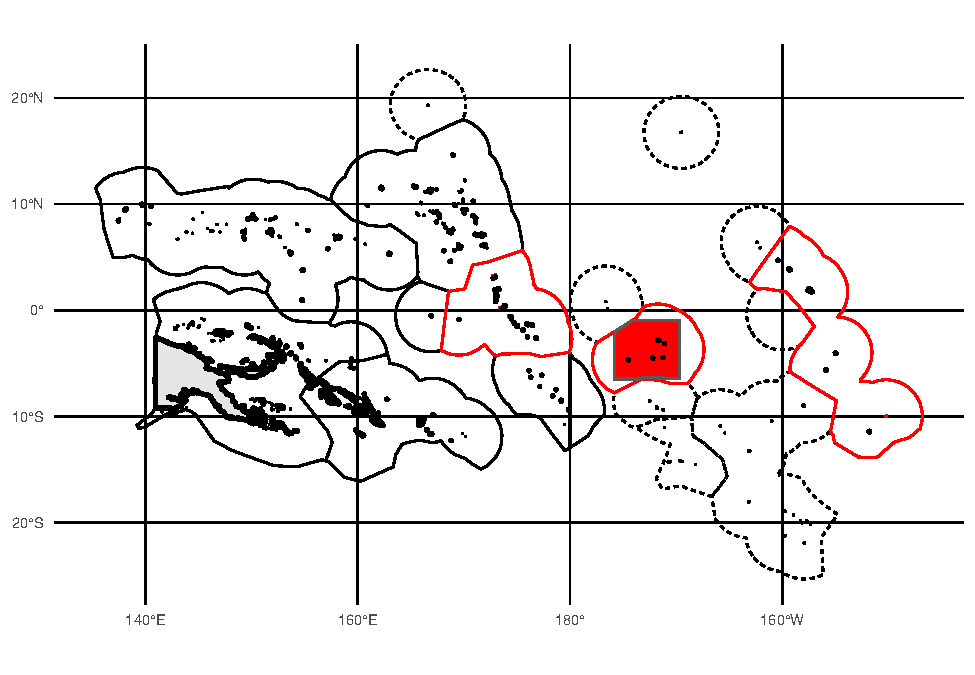
\includegraphics{C:/Users/JC/Documents/GitHub/MPA_displacement/docs/Manuscript_files/figure-latex/unnamed-chunk-3-1.pdf}
\caption{\label{fig:unnamed-chunk-3}\label{fig:PNA_map}Map of the Exclusive
Economic Zones (EEZs) of the region of interest. A solid line indicates
countries that belong to the PNA, while a dashed line indicates all
others. A red line indicates the Kiribati EEZ, and a solid red polygon
delineates PIPA.}
\end{figure}

The main tuna species caught in the region are skipjack
(\emph{Katsuwonus pelamis}), yellowfin (\emph{Thunnus albacares}),
albacore (\emph{Thunnus alalunga}) and bigeye (\emph{Thunnus obesus}).
From these, the first two are amongst the top-10 species represented in
global fisheries production statistics, with 2016 catches increasing
relative to the 2005-2014 average \citep{fao_2018}. Theis region of the
Pacific has historically accounted for a large portion of tuna catches
\citep{aqorau_1997}. Today, the PNA controls close to 50\% of the global
skipjack tuna production \citep{pna_website_2018}. A large portion of
these catches derive from purse seine vessels licensed under the VDS.
Fishing vessels from Australia, New Zeland, China, France, Korea, Japan,
the Philippines, Taiwan, and the United States participate in the
purse-seining VDS.

One of the most notable and recent management interventions in the
region is the implementation of the Phoenix Island Protected Area (PIPA)
by the government of Kiribati. PIPA was first declared in 2006, and
established in 2008 with only 4\% of it was declared as no-take. In
January 1\textsuperscript{st}, 2015, the no-take area within PIPA was
expanded to a total area of 397,447 km\textsuperscript{2}, roughly 1.5
times the size of Ecuador. Figure \ref{fig:PNA_map} shows a map of the
PNA countries and the Phoenix Island Protected Area.

The closure of such a large area in one of the most important fishing
regions in the world provides a great opportunity to evaluate the
behavioral responses and redistribution of fishing effort by vessels
that used to fish there. PIPA has been the focus of previous research,
showing that fishing effort is effectively reduced after implementation
\citep{mccauley_2016,mcdermott_2018}. To this, we pose two questions:
How do individual vessels respond to the sudden exclusion of such a big
area? And where did all the vessels go? In the next sections we describe
the data and methods used to answer this questions.

\hypertarget{methods}{%
\section{Methods}\label{methods}}

This section is divided into two main parts. First, we provide a general
description of AIS data and the process of identification of
vessel-level fishing events done by Global Fishing Watch\footnote{Global
  Fishing Watch: \url{globalfishingwatch.org}}. Alongside, we describe
the subset of data used on our analyses. When relevant, we also point
out possible shortcomings in the data, or factors that must be
considered in the later analyses. We then move on to explain our
empirical strategy for the identification of the behavioral changes and
redistribution of fishing effort.

\hypertarget{data}{%
\subsection{Data}\label{data}}

Automatic Identification Systems (AIS) are on-board devices that provide
at-sea safety and prevent ship collisions by broadcasting vessel
position, course, and activity to surrounding vessels. These broadcasted
messages can be received by satellites and land-based antennas. GFW uses
convolutional neural networks to infer vessel characteristics and
whether each broadcasted position represents a fishing event, thus
allowing us to estimate near real-time fishing events globally since
2012 \citep{kroodsma_2018}.

The amount of data gathered is dependent on the number of antennas and
satellites that can pick up the signals. In June 1\textsuperscript{st}
2014 satellite count increased from 3 to 6, and then to 10 in January
1\textsuperscript{st} 2016. This causes an increase in the number of
\emph{received} AIS messages (\emph{i.e.} points), and therefore an
apparent increase in the number of vessels and fishing hours. However,
the addition of satellites ``affects'' all vessels in the same way. The
variability in AIS data and ocean conditions require that temporal
trends be taken into account. We do that by including specific controls
in our identification strategy and using a subset of data that meet a
BACI design -which gives us the full tracks for vessels affected and
unaffected by the implementation of PIPA.

Our analysis focuses on purse seine vessels, the most important fishery
for PNA
countries\footnote{We perform some of the same analyses for longliners and include them in the Appendix}.
We identify a total of 103 purse seiners that fished in PNA waters at
least once before
2015\footnote{New vessels that entered the fishery after 2015 were not exposed to the policy intervention in the pre-treatment period and are therefore exlcuded from our analyses.}.
These vessels represent over 26 million individual observations for the
2012 - 2017 period. We identify 65 vessels that have fished inside PIPA
at least once since 2012. From these, 62 did so before the anouncement
(\emph{i.e.} 09/01/2014 \emph{sensu} \citep{mcdermott_2018}) but are
only able to track 61 for the complete periof of study before and after
its
implementation\footnote{1 vessel never fished again after August 18, 2013.}.
On the other hand, 38 vessels never fished inside PIPA but we only have
data for 26 vessels before and after.

Therefore, our treatment group contains all purse seiners (n = 61) that
fished within PIPA at least once before the anouncement, and that
continued to fish elsewhere after the January 2015 implementation.
Vessels in the control group meet the following two conditions: i)
vessels never fished within PIPA waters, and ii) vessels have fished in
surrounding areas (\emph{i.e.} PNA-countries' EEZ) before and after PIPA
closure (n = 26).

We include three additional definitions of control groups as a
robustness check: one with only vessels that belong to PNA countries (n
= 7), and one that excludes Chinese vessels (n = 21). Our third control
is made up of Japanese purse seiners that fish in the Pacific but that
never fished inside PIPA (n =
27)\footnote{Using Taiwanese vessels was the original idea, but there are only 4 vessels with pre-2015 data. I need to further identify propper Taiwanese vessels, as I am currently using the entire Pacific ocean}.
Our definition of treatment and control groups leaves us with 61 and 21
treated and control vessels, which have just over 22 million
observations where about 22\% are identified as fishing events.

For each vessel we calculate total daily fishing hours and obtain pannel
data with 37,800 observations. Table \ref{tab:baci_n_s} shows the number
of vessels following a BACI design, as well as the fishing hours, before
and after PIPA. Fig. \ref{fig:all_vessels} shows that mean fishing hours
for purse seiners have an abrupt increase, just before January 1st,
2015. This trend is observed for both treated and control groups. Across
all measures, the treatment and control vessels follow similar patterns,
confirming our claim that the control group provides a plausible
counterfactual. Figure \ref{fig:baci_strict} provides a visual
representation of the vessel-level fishing events that make up each
group through time. We use this data to answer our key questions: How do
the 61 purse seiners modify their behavior as compared to the different
control groups, and where do they go after the spatial closure? The
following section describes our empirical identification strategies.

\begin{table}[H]

\caption{\label{tab:unnamed-chunk-6}\label{tab:baci_n_s}Number of fishing vessels and mean daily fishing hours by group before and after PIPA implementation.}
\centering
\begin{tabular}[t]{lrrrr}
\toprule
Group & n & Before & After & Change (A / B)\\
\midrule
Control & 26 & 11.74 & 20.13 & 1.72\\
Treatment & 61 & 10.67 & 18.36 & 1.72\\
\bottomrule
\end{tabular}
\end{table}

\begin{figure}
\centering
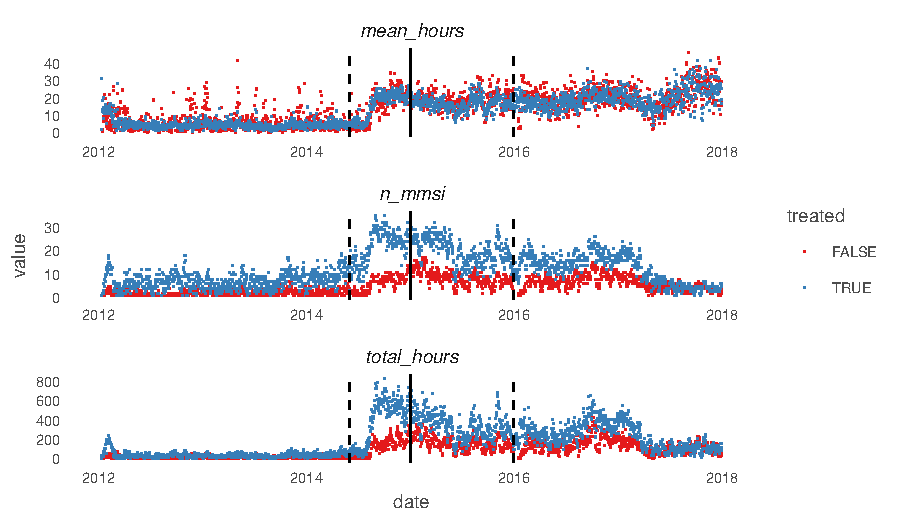
\includegraphics{C:/Users/JC/Documents/GitHub/MPA_displacement/docs/Manuscript_files/figure-latex/unnamed-chunk-7-1.pdf}
\caption{\label{fig:unnamed-chunk-7}\label{fig:all_vessels}Fishing hours and
number of vessels by month for all vessels. Vertical dashed lines
indicates dates when satellites were added, solid line indicates PIPA
closurePIPA closure.}
\end{figure}

\hypertarget{analyses}{%
\subsection{Analyses}\label{analyses}}

The first analysis focuses on identifying the response of fishing
vessels to PIPA closure. A spatial closure might cause fishers to modify
their behavior as they adapt to a new state of the world. Some may have
to travel further distances to find new fishing grounds, which would
lead them to fish harder to compensate for the associated extra fuel
costs. If fishers had developed experience for fishing in particular
sites, being excluded might impose a learning cost on them, as they
identify new fishing grounds. This would result in increased search
times. However, if the area of influence of a vessel is significantly
larger than that of the spatial closure, they might already know other
places and times where to fish. Our variables of interests intend to
caputre these possible reactions.

We use daily fishing hours, daily proportion of fishing vs.~non-fishing
hours, and daily distance traveled (km). We compare our variable of
interest before and after the implementation of PIPA using a
Difference-in-Differences approach, where we track the variable of
interest for vessels described in the previous section. Our
specification is the following:

\[
y_{i,t} = \alpha + \beta_1 Post_t + \beta_2 Treat_i + \beta_3 Post_t \times Treat_i + \phi_t + \gamma_i + \epsilon_{i,t}
\]

Where \(y_{i,t}\) is the variable of interest for vessel \(i\) in time
period \(t\). A dummy variable \(Post_t\) takes the value of 0 for all
dates prior to PIPA implementation and a value of 1 for all dates
including and following PIPA implementation. \(Treat_i\) is a dummy
variable indicating whether a vessel belongs to the control
(\(Treat_i = 0\)) or treatment (\(Treat_i = 1\)) group. \(\alpha\) is
the standard intercept, \(\beta_1\) captures the temporal trend change,
\(\beta_2\) captures the difference between treated and control groups,
and \(\beta_3\) is our parameter of interest: de DiD estimate capturing
the treatment effect. Finally, \(\phi_t\) and \(\gamma_i\) represent
month-, and flag-level dummies that account for seasonality or
country-level management
interventions\footnote{We test for other more complex specifications that interact a quarterly dummy or year-month dummies with the treatment group and find qualitatively the same results.}.

Our second part of the analyses focuses on the redistribution of fishing
effort. The role of institutions may play an important role. As stated
before, LSMPAs often span the entirety of an EEZ. In the case of purse
seining in the PNA, vessels purchase access to the fishery at the
beginning of the season. If a vessel decides to fish within the PNA,
they've already made the decission to pay for access, expecting higher
returns from fishing there than in the High Seas. In the particular case
of PIPA, one would expect that a vessel holding a permit to fish in
I-Kiribati waters would then move to other fishing grounds within
Kiribati after the closure. Alternatively, if a vessel fishes illegaly
in I-Kiribati waters before the implementation, one would expect them to
reallocate to other regions with equal or less enforcement. In this
case, they might then choose to move to other I-Kiribati waters, waters
of countries that have similar enforcement levels, or the High Seas.

We discretize spatial units by using a polygon for PIPA
\footnote{we would expect to see a decrease here} and distinct spatial
units for each EEZ of each country. Some vessels might shift from EEZs
into the high seas, but we are interested in knowing \emph{where} in the
high seas, so we incorporate additional regions by using a 1 degree
buffer of the high seas arround each of the EEZ regions. The rest of the
high seas are merged into a single spatial unit. For example, if we were
to do this only for Kiribati, we would have 8 spatial units: PIPA, three
EEZs, three 1-degree buffers of high seas arround each EEZs, and the
rest of the high seas. Whenever the buffers overlapped between
themselves, we randocmply clipped one on to the other. EEZs that had
sporadic fishing events were pooled into a group of ``others''.

To evaluate this change in effort allocation, we regress our variable of
interest (\emph{i.e.} fishing hours) on the interaction between a dummy
variable indicating the policy intervention and a dummy variable for
countries. This gives us the by-country change in proportional
allocation of fishing effort:

\[
y_{i,t} = \alpha + \beta_1Post + \beta_{2,i}Country + \beta_{3,i}Post_t \times Country_i + \epsilon_{i,t}
\]

Our variable of interest, \(y_{i,t}\) represents the proportion of
fishing hours that country \(i\) receives at time \(t\). \(Post\) also
represents a policy dummy that takes the value of 0 for all dates before
implementation of PIPA, and 1 otherwise. \(Country\) is a dummy variable
for countries for the spatial units defined above. Our parameter of
interest is \(\beta_{1,i}\), which captures the country-level change in
proportional fishing effort.

All regression coefficients were estimated via ordinary least squares,
and heteroskedastic-robust standard errors were calculated. All analyses
were performed in R version 3.5.1 \citep{rcore_2018}. Raw data and code
used in this work are available on
\href{https://github.com/jcvdav/MPA_displacement}{github}.

\begin{table}[H]

\caption{\label{tab:unnamed-chunk-9}\label{tab:ba_disp}Changes in the relative allocation of fishing effort by region (EEZ, PIPA, high seas) and gear.}
\centering
\begin{tabular}[t]{lr}
\toprule
country & change\\
\midrule
EEZ COK 1 & 0.53\\
EEZ FSM 1 & 0.81\\
EEZ KIR 1 & -0.16\\
EEZ KIR 2 & 4.50\\
EEZ KIR 3 & -2.79\\
\addlinespace
EEZ MHL 1 & -0.44\\
EEZ NRU 1 & 0.07\\
EEZ PNG 2 & -9.07\\
EEZ SLB 1 & 3.18\\
EEZ TUV 1 & 1.27\\
\addlinespace
HS & 3.93\\
HS COK 1 & 0.06\\
HS KIR 1 & 2.96\\
HS KIR 2 & 1.07\\
HS KIR 3 & 2.53\\
PIPA PIPA 1 & -8.25\\
\bottomrule
\end{tabular}
\end{table}

\clearpage

\hypertarget{results}{%
\section{Results}\label{results}}

Our DiD analysis shows an overall increase in purse seine fishing hours,
even after accounting for the introduction of new satellites (Table
\ref{tab:did}). This coefficient estimate is consistent for different
model specifications and across groups of treatment and controls. These
effectively represent the patterns observed in Figure
\ref{fig:all_vessels}. The \(\beta_3\) coefficient indicating our
treatment effect suggests that, relative to the control, treated vessels
fish less, in the order of 0.5 hours per day. Another way to interpret
this is that the increase in fishing effort by treated vessels has
ocurred at a lower rate than control vessels. This result is robust and
significant (\(p < 0.05\)) for all model specifications using our main
control group, with the effect varying between \(\beta_3 = -0.515\) and
\(\beta_3 = -0.934\). These values are equivalent to a 15 - 28 reduction
in fishing hours per month.

Regressions coefficients for our DiD analysis are shown in Table
\ref{tab:did}. Columns 1 -3 use all data for controls. Columns 4 - 6 use
only PNA vessels as controls, and columns 7 - 9 exclude Chinese vessels.
Columns 10 and 11 use Japanese vessels in the Pacific as controls, and
hence don't include flag FEs to avoid perfect colinearity between
Japanese flag and
control\footnote{Results of the same analysis is shown for longliners in \ref{tab:long}}.
It must be noted, however, that when reducing the linear structure of
the \(Pre \times Post\) design and instead interacting the treatment
dummy with quarterly or year-month combinations we are not able to
reject the null hypotheses of no change (Figures
\ref{fig:q1,fig:q2,fig:q3,fig:q4,fig:ym1,fig:ym2,fig:ym3,fig:ym4}).

\begin{figure}
\centering
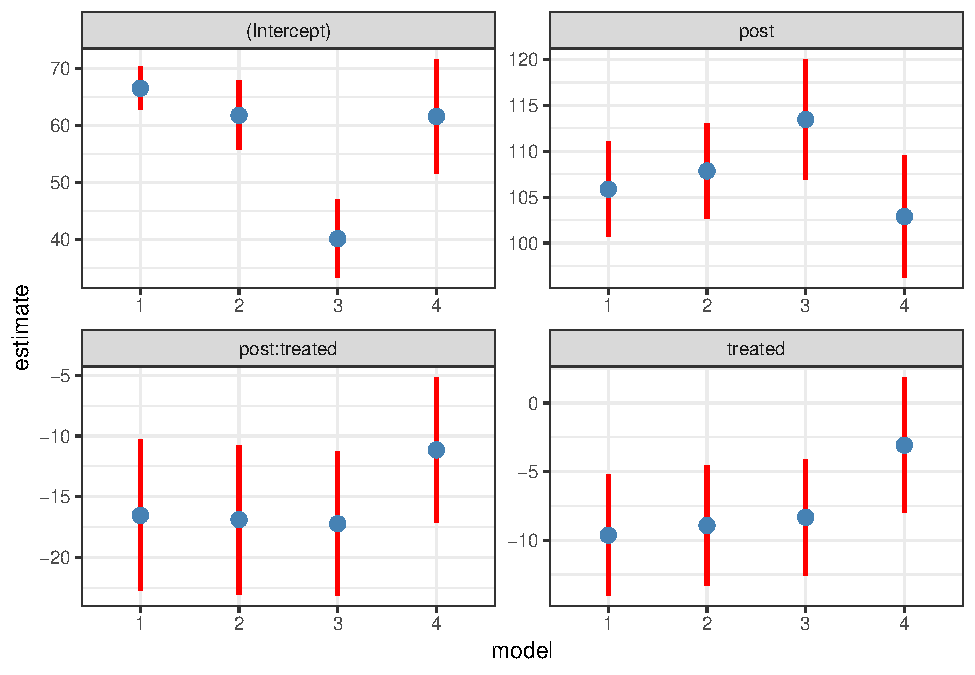
\includegraphics{C:/Users/JC/Documents/GitHub/MPA_displacement/docs/Manuscript_files/figure-latex/unnamed-chunk-10-1.pdf}
\caption{\label{fig:unnamed-chunk-10}\label{fig:all_vessels}Daily fishing
hours for all vessels in our main treatment-control groups. Solid
straight lines show a linear trend by period (pre-psot) and treatment.
The other red and blue lines show monthly avarages. Vertical dashed line
indicates PIPA closure.}
\end{figure}

\clearpage
\begin{landscape}


\begin{table}[!htbp] \centering 
  \caption{\label{tab:did}Difference-in-differences estimates for 3 different controls and 3 different specifications. The first three columns use all data for controls. Columns 4 - 6 use only PNA vessels as controls, and columns 7 - 9 exclude Chinese vessels. Columns 10 and 11 use Japanese vessels in the Pacific as controls, and hence don't include flag FEs. Numbers in parentheses are heteroskedastic-robust standard errors.} 
  \label{} 
\footnotesize 
\begin{tabular}{@{\extracolsep{1pt}}lccccccccccc} 
\\[-1.8ex]\hline 
\hline \\[-1.8ex] 
 & \multicolumn{11}{c}{\textit{Dependent variable:}} \\ 
\cline{2-12} 
\\[-1.8ex] & \multicolumn{11}{c}{hours} \\ 
\\[-1.8ex] & (1) & (2) & (3) & (4) & (5) & (6) & (7) & (8) & (9) & (10) & (11)\\ 
\hline \\[-1.8ex] 
 Constant & 6.345$^{***}$ & 7.863$^{***}$ & 10.322$^{***}$ & 7.124$^{***}$ & 9.007$^{***}$ & 9.933$^{***}$ & 6.057$^{***}$ & 7.584$^{***}$ & 10.194$^{***}$ & 22.625$^{***}$ & 24.731$^{***}$ \\ 
  & (0.186) & (0.274) & (0.404) & (0.265) & (0.341) & (0.620) & (0.193) & (0.279) & (0.538) & (0.629) & (0.683) \\ 
  & & & & & & & & & & & \\ 
 post & $-$0.052 & 1.134$^{***}$ & 1.115$^{***}$ & $-$1.199$^{***}$ & $-$0.279 & 0.124 & $-$0.284 & 1.013$^{***}$ & 1.166$^{***}$ & 2.330$^{***}$ & 3.991$^{***}$ \\ 
  & (0.303) & (0.304) & (0.339) & (0.435) & (0.429) & (0.436) & (0.318) & (0.318) & (0.357) & (0.890) & (0.877) \\ 
  & & & & & & & & & & & \\ 
 treated & $-$1.142$^{***}$ & $-$0.839$^{***}$ & 0.010 & $-$1.977$^{***}$ & $-$1.675$^{***}$ & 0.626 & $-$0.877$^{***}$ & $-$0.536$^{**}$ & 0.150 & $-$18.190$^{***}$ & $-$18.257$^{***}$ \\ 
  & (0.214) & (0.209) & (0.281) & (0.284) & (0.274) & (0.416) & (0.221) & (0.215) & (0.297) & (0.673) & (0.661) \\ 
  & & & & & & & & & & & \\ 
 sate2 & 12.579$^{***}$ & 11.589$^{***}$ & 11.340$^{***}$ & 12.709$^{***}$ & 11.850$^{***}$ & 11.749$^{***}$ & 12.631$^{***}$ & 11.599$^{***}$ & 11.349$^{***}$ & 14.346$^{***}$ & 12.967$^{***}$ \\ 
  & (0.197) & (0.199) & (0.232) & (0.212) & (0.213) & (0.246) & (0.199) & (0.201) & (0.235) & (0.303) & (0.309) \\ 
  & & & & & & & & & & & \\ 
 sate3 & 14.675$^{***}$ & 13.587$^{***}$ & 13.328$^{***}$ & 14.799$^{***}$ & 13.894$^{***}$ & 13.795$^{***}$ & 14.958$^{***}$ & 13.804$^{***}$ & 13.566$^{***}$ & 15.187$^{***}$ & 13.719$^{***}$ \\ 
  & (0.260) & (0.262) & (0.307) & (0.286) & (0.287) & (0.329) & (0.264) & (0.266) & (0.315) & (0.402) & (0.410) \\ 
  & & & & & & & & & & & \\ 
 post:treated & $-$0.515$^{*}$ & $-$0.833$^{***}$ & $-$0.934$^{***}$ & 0.562 & 0.373 & $-$0.176 & $-$0.439 & $-$0.814$^{***}$ & $-$1.084$^{***}$ & $-$3.209$^{***}$ & $-$3.715$^{***}$ \\ 
  & (0.281) & (0.276) & (0.310) & (0.413) & (0.402) & (0.407) & (0.293) & (0.287) & (0.326) & (0.811) & (0.799) \\ 
  & & & & & & & & & & & \\ 
\hline \\[-1.8ex] 
Control & All & All & All & PNA & PNA & PNA & -CHN & -CHN & -CHN & JPN & JPN \\ 
Month FE & No & Yes & Yes & No & Yes & Yes & No & Yes & Yes & No & Yes \\ 
Flag FE & No & No & Yes & No & No & Yes & No & No & Yes & No & No \\ 
Observations & 37,840 & 37,840 & 30,359 & 30,583 & 30,583 & 25,034 & 36,415 & 36,415 & 28,934 & 34,047 & 34,047 \\ 
R$^{2}$ & 0.171 & 0.200 & 0.208 & 0.178 & 0.208 & 0.215 & 0.173 & 0.203 & 0.211 & 0.260 & 0.280 \\ 
\hline 
\hline \\[-1.8ex] 
\textit{Note:}  & \multicolumn{11}{r}{$^{*}$p$<$0.1; $^{**}$p$<$0.05; $^{***}$p$<$0.01} \\ 
\end{tabular} 
\end{table} 

\end{landscape}
\clearpage

\begin{figure}
\centering
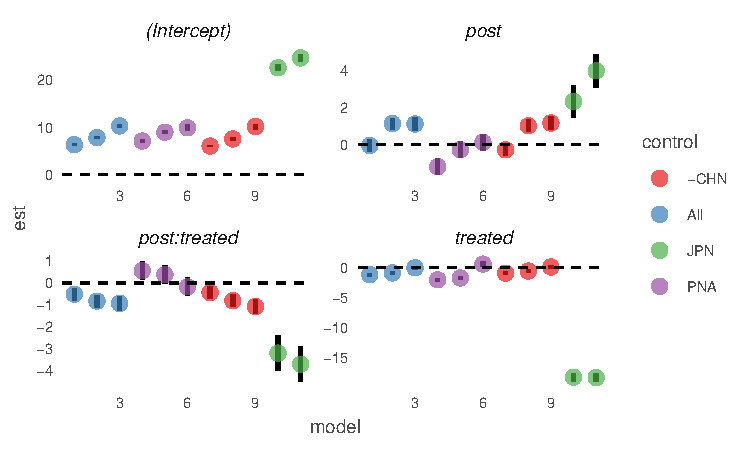
\includegraphics{C:/Users/JC/Documents/GitHub/MPA_displacement/docs/Manuscript_files/figure-latex/unnamed-chunk-12-1.pdf}
\caption{\label{fig:unnamed-chunk-12}\label{fig:long}Coefficient estimates
for each model. Top pannel indicates variable, x-axis represents model
specification, and y-axis coefficient estimate.}
\end{figure}

Recall that to evaluate the redistribution of fishing effort we only
track fishing vessels that belong to the treated group. Figure
\ref{fig:fishing_raster} provides a spatial representation of these
changes. Note that 2013 effort distribution is roughly similar across
vessels. Then in 2014 there is a sharp increase in fishing hours by
treated vessels inside PIPA (blue paradox). In 2015 treated vessels then
allocate more effort to the easternmost Kiribati EEZ (see Figure
\label{fig:PNA_map}) and the high seas. In 2016 spatial distribution of
fishing effort is again similar across groups. It is evident that the
increase in relative fishing effort is greater for for regions closer to
PIPA, and.

Four our empirical identification we calculated the proportion of
fishing effort allocated every month to each spatially explicit regions
defined in section \ref{methods}. For purse seiners, these represent 9
main EEZs, PIPA, the high seas, and a group of other EEZs. Figure
\ref{fig:redist_trend_ps} shows the monthly relative fishing hours that
each region received by all 61 treated vessels. The top-left panel shows
the change in fishing effort inside PIPA, including the preemptive
fishing and immediate reduction previously reported
\citep{mcdermott_2018}. The change in the relative allocation of fishing
effort by purse seiners increases in eight of the 12 regions after PIPA
implementation (Table \ref{tab:disp_mod}, fig:map\_change\_ps). The
largest increase is observed for the I-Kiribati EEZ, with an average
increase of 0.11 (\emph{p \textless{} 0.001}). In other words, the
redistribution of treated vessels caused a 10\% increase in the
\emph{relative} allocation of fishing effort within I-Kiribati waters.
The only decrease is observed for Papua New Guinea, but the coefficient
is not significant.

\begin{figure}
\centering
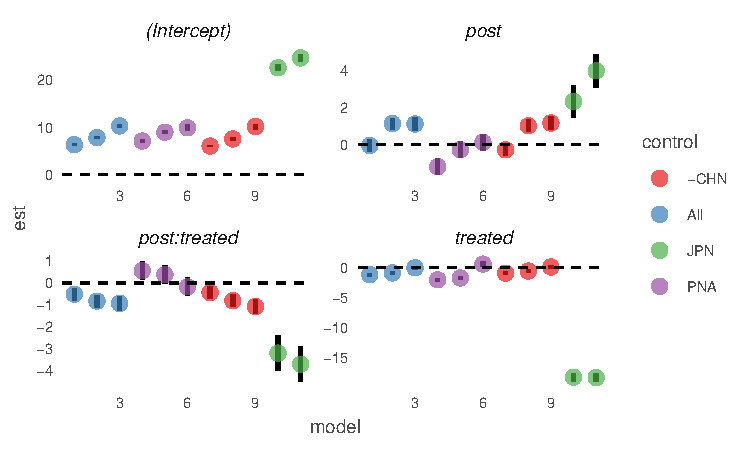
\includegraphics{C:/Users/JC/Documents/GitHub/MPA_displacement/docs/Manuscript_files/figure-latex/unnamed-chunk-13-1.pdf}
\caption{\label{fig:unnamed-chunk-13}\label{fig:fishing_raster}Yearly
spatial distribution of fishing effort by treated and control vessels.
Colors have been adjusted relative to the maximum observed by group and
year.}
\end{figure}

\begin{figure}
\centering
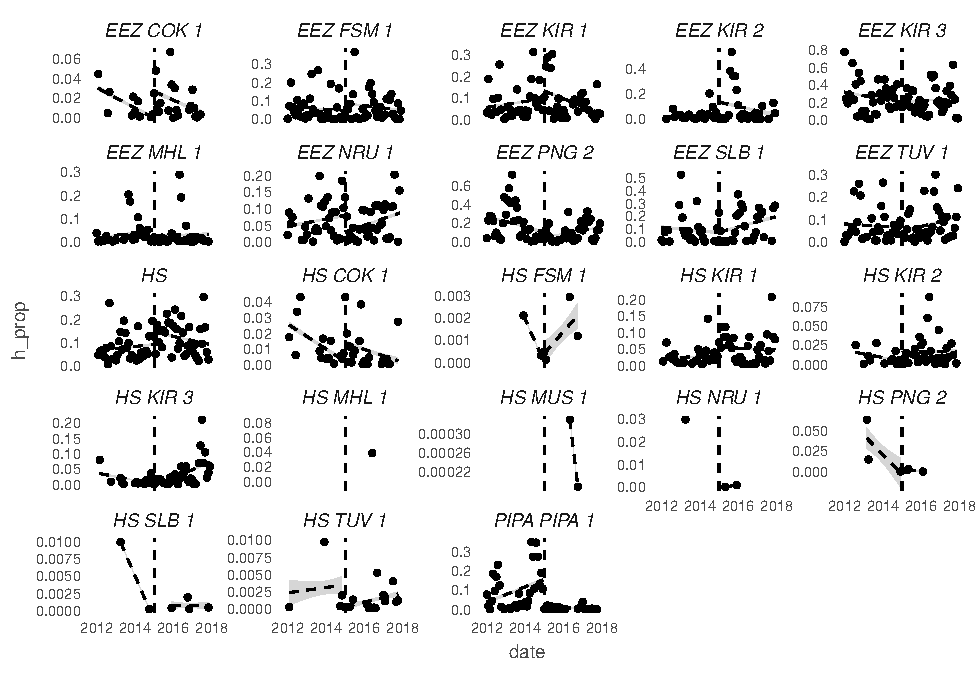
\includegraphics{C:/Users/JC/Documents/GitHub/MPA_displacement/docs/Manuscript_files/figure-latex/unnamed-chunk-14-1.pdf}
\caption{\label{fig:unnamed-chunk-14}\label{fig:redist_trend_ps}Monthly
relative allocation of fishing effort by PIPA-fishing vessels before and
after PIPA for 9 EEZs, PIPA, the high seas and `other EEZs'.}
\end{figure}

\begin{figure}
\centering
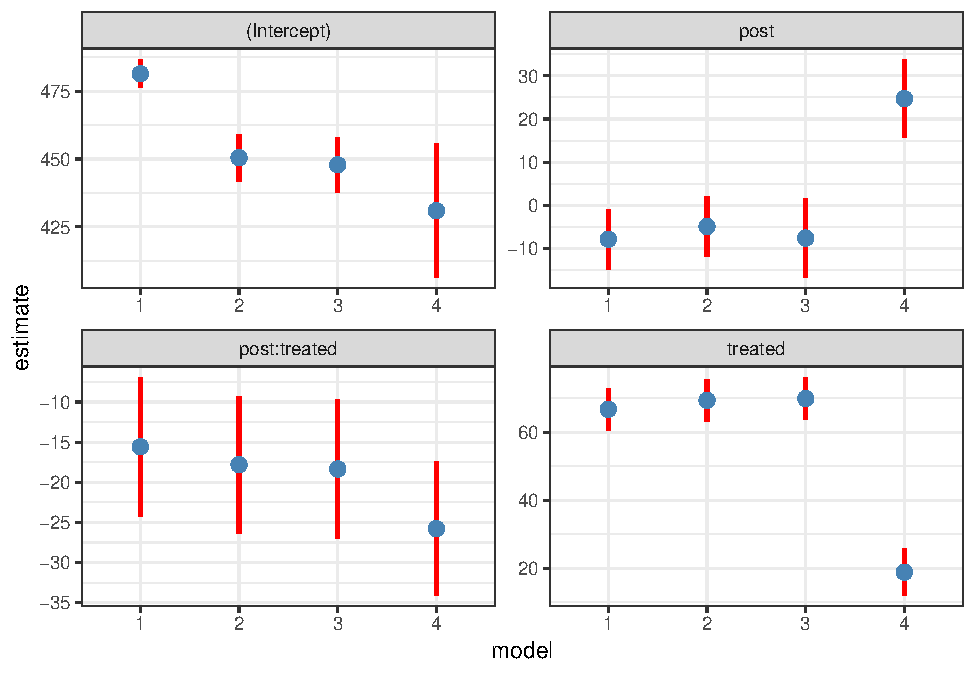
\includegraphics{C:/Users/JC/Documents/GitHub/MPA_displacement/docs/Manuscript_files/figure-latex/unnamed-chunk-15-1.pdf}
\caption{\label{fig:unnamed-chunk-15}\label{fig:map_change_ps}Spatial
representation of the mean change in the monthly allocation of fishing
effort for purse seiners.}
\end{figure}

\begin{table}[H]

\caption{\label{tab:unnamed-chunk-16}\label{tab:disp_mod}Change in the relative allocation of purse seining fishing hours by region (R2 = 0.36, F(47, 69000) = 961.1, p < 0.001)}
\centering
\begin{tabular}[t]{ll}
\toprule
term & h\_prop\\
\midrule
(Intercept) & 0.087 (0.002)***\\
post & -0.081 (0.003)***\\
sate2 & -0.003 (0.001)***\\
sate3 & -0.002 (0.001)\\
post:countryEEZ COK 1 & 0.088 (0.002)***\\
\addlinespace
post:countryEEZ FSM 1 & 0.091 (0.003)***\\
post:countryEEZ KIR 1 & 0.081 (0.003)***\\
post:countryEEZ KIR 2 & 0.127 (0.004)***\\
post:countryEEZ KIR 3 & 0.055 (0.005)***\\
post:countryEEZ MHL 1 & 0.078 (0.003)***\\
\addlinespace
post:countryEEZ NRU 1 & 0.083 (0.003)***\\
post:countryEEZ PNG 2 & -0.008 (0.005)*\\
post:countryEEZ SLB 1 & 0.114 (0.004)***\\
post:countryEEZ TUV 1 & 0.095 (0.003)***\\
post:countryHS & 0.122 (0.003)***\\
\addlinespace
post:countryHS COK 1 & 0.083 (0.002)***\\
post:countryHS KIR 1 & 0.112 (0.003)***\\
post:countryHS KIR 2 & 0.093 (0.002)***\\
post:countryHS KIR 3 & 0.108 (0.003)***\\
\bottomrule
\end{tabular}
\end{table}

\clearpage

\hypertarget{discussion}{%
\section{Discussion}\label{discussion}}

Our findings provide interesting insights into the effect that LSMPAs
can have on vessel behavior and the redistribution of fishing effort.
These collection of results shows that the implementation of PIPA caused
treated vessels to reduce their fishing hours, and that this effect is
greater for purse seiners than longliners. Even though treated vessels
fish less, their relative allocation of fishing hours increased for all
other fishing grounds. This does not imply that there is more fishing
effort exerted by treated vessels, but rather that each region receives
a greater portion of the post-PIPA fishing effort of these same vessels,
which is lower than pre-PIPA levels. In this section we discuss the
implications of vessel-level reductions in fishing effort and the
increase in relative allocation of the remaining effort through space.
We also provide plausible explanations as to why purse seiners seem to
be more reactive to the spatial closure.

A major shortcoming of our analyses is that we do not observe catches or
revenues, which ultimately are the factors that guide the decision
making process of profit-maximizing agents. Therefore, it is difficult
to know whether the reduction in fishing effort represents a positive or
negative impact. A decrease in fishing effort is associated to an
increase in catches (and therefore greater CPUE) only when the entire
fleet does it, and if previous levels of effort were greater than
\(F_{MEY}\) (\emph{i.e.} the effort that would yield the maximum
economic yield). Therefore, it is plausible that the reduction of
fishing hours is not done by choice, but rather results from fishers
having to increase search time. Upon being relocated, fishers may not
identify the best fishing grounds as easily as before, and therefore
invest a greater proportion of their time searching for their catch.
Further analysis of temporal trends in non-fishing hours, as well as
distance traveled should provide us with insights as to why fishers
reduced fishing hours.

Previous studies on insular environments suggest that vessels move to
distant places, which might be translated as increased costs
\citep{stevenson_2013}. Nevertheless, they do not use counterfactuals
that could help account for system- or fleet-level changes that occur
through time. Others have used similar satellite-tracking systems to
show that fishing effort accumulates near the edges of spatial closures,
yielding greater catches \citep{murawski_2005}. Yet, these vessel tracks
do not cover the pre-reserve period, making it difficult identify the
contribution of spatial closures to the observed spatial distribution of
fishing vessels. Recent work by \citet{elahi_2018} identified that total
fishing effort in a focal region where a short-term MPA was implemented
showed little change, likely indicating that fishers redistributed
fishing effort to compensate for the reduction in available space. Our
data is assembled in a similar way, with fishing positions before and
after the implementation of PIPA and vessels grouped into treated and
control groups. Our BACI design, along with our
difference-in-differences analysis allows us to make causal inferences
about the effect that large scale marine protected areas have on fishing
effort.

The different responses observed between purse seiners and longliners
might have two possible explanations. It is likely that PIPA did not
contain habitat that longliners would consider optimal. Therefore, the
sporadic fishing events that occurred there are of little importance to
the fleet, and it is unlikely that the implementation of PIPA has an
effect on them. Alternatively, the differences may be due to the nature
of each fishing gear. Purse seiners are often constrained by seafloor
and termocline depth, and have a smaller spatial footprint
\citep{kroodsma_2018}. Tuna purse seiners are known to have greater
proportion of null sets (\emph{i.e.} where purse seines effectively cast
their nets, but no catch is obtained) during El Niño years, where the
termocline deepens in the Eastern Pacific \citep{dreyfusleon_2015}. On
the other hand, longliners may be more flexible as to where they can
deploy their longlines. \citet{ortuocrespo_2018} evaluated the
ecological niche of the pelagic longline fleet, and suggest that the
fleet may be under-utilizing the ocean, meaning that they can easily
redistribute elsewhere.

Our work suggests that the implementation of LSMPAs can have important
implications for purse seiners, and less so for longliners. We also show
that fishing effort is redistributed to areas close by. Future
management interventions that aim to close large portion of the oceans
should consider how fishing effort will change in space and through
time, and the ecological implications of this redistribution to ensure
that fishing effort is not just displaced elsewhere, leading to
overfishing in adjacent waters.

Furthermore, a growing body of literature suggests that closing the high
seas to all fishing could increase fishery yields and profitability of
fisheries, with negligible costs to food security
\citep{white_2014,sumaila_2015,sala_2018a,schiller_2018}.

\clearpage

\hypertarget{refs}{}

\clearpage

\hypertarget{appendix}{%
\section{Appendix}\label{appendix}}

\setcounter{table}{0}  \renewcommand{\thetable}{S\arabic{table}} \setcounter{figure}{0} \renewcommand{\thefigure}{S\arabic{figure}}

\hypertarget{stream-of-data-by-vessel-group-and-period}{%
\subsection{Stream of data by vessel, group, and
period}\label{stream-of-data-by-vessel-group-and-period}}

\begin{figure}
\centering
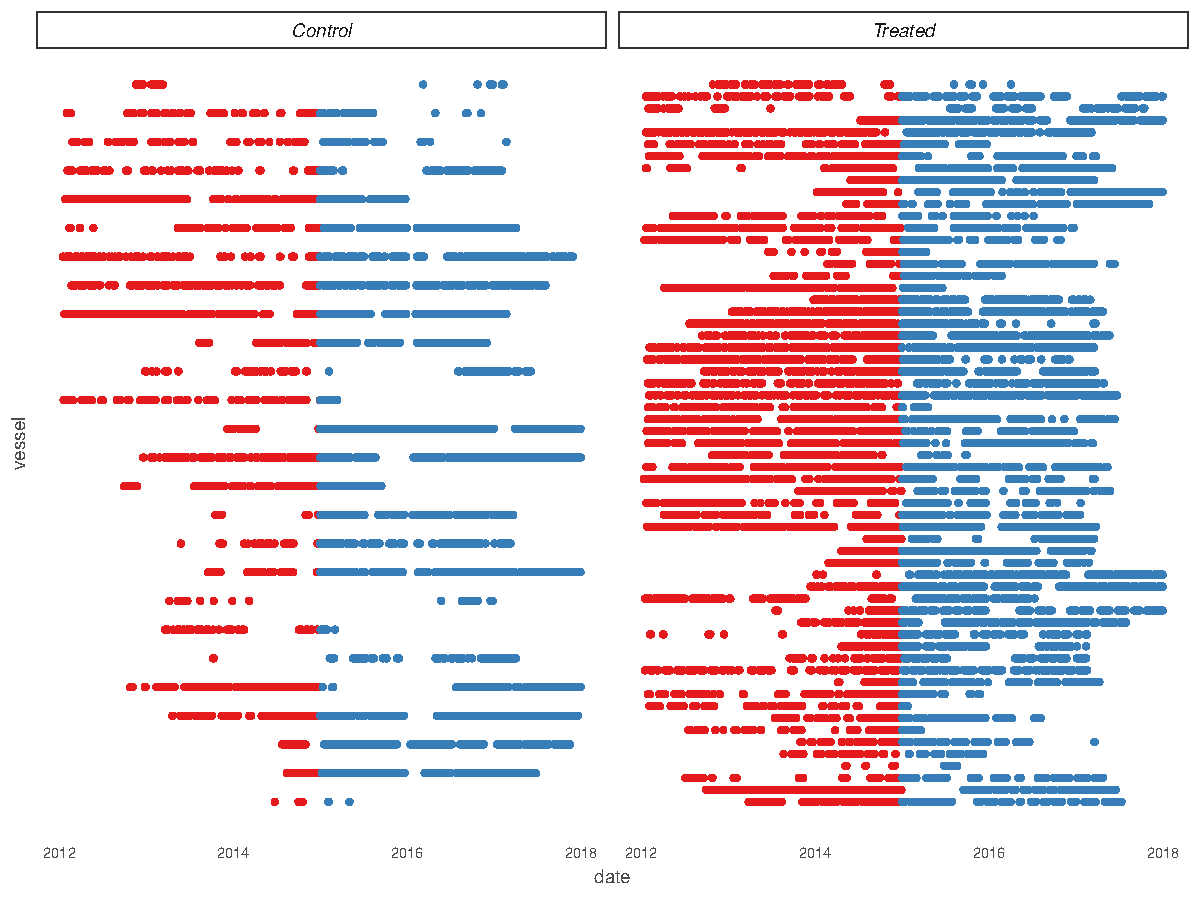
\includegraphics{C:/Users/JC/Documents/GitHub/MPA_displacement/docs/Manuscript_files/figure-latex/unnamed-chunk-17-1.pdf}
\caption{\label{fig:unnamed-chunk-17}\label{fig:baci_strict}Stream of
fishing events by vessels through time. Each line represents a vessel,
with dots indicating months with fishing activity and colors indicating
the pre and post periods.}
\end{figure}

\clearpage

\hypertarget{longliners}{%
\subsection{Longliners}\label{longliners}}

Longliners show a similar pattern of effort reduction. However, the
magnitude of the \(\beta_3\) coefficient is smaller (ranging from
\(\beta_3 = -0.98\) to \(\beta_3 = -1.125\)) and not significant unless
including month and flag FEs for the general treatment-control groups,
or when excluding Chinese vessels. This, along with higher standard
error values suggest that longliners have a smaller and more variable
response to the implementation of LSMPAs.

\begin{table}[!htbp] \centering 
  \caption{\label{tab:long}Difference-in-differences estimates for 2 different controls and 3 different specifications. The first three columns use all data for controls. Columns 4 - 6 exclude Chinese vessels. Numbers in parentheses are heteroskedastic-robust standard errors.} 
  \label{} 
\small 
\begin{tabular}{@{\extracolsep{1pt}}lcccccc} 
\\[-1.8ex]\hline 
\hline \\[-1.8ex] 
 & \multicolumn{6}{c}{\textit{Dependent variable:}} \\ 
\cline{2-7} 
\\[-1.8ex] & \multicolumn{6}{c}{hours} \\ 
\\[-1.8ex] & (1) & (2) & (3) & (4) & (5) & (6)\\ 
\hline \\[-1.8ex] 
 Constant & 39.192$^{***}$ & 38.411$^{***}$ & 36.520$^{***}$ & 39.402$^{***}$ & 38.636$^{***}$ & 34.402$^{***}$ \\ 
  & (0.095) & (0.132) & (0.169) & (0.102) & (0.140) & (0.236) \\ 
  & & & & & & \\ 
 post & $-$1.014$^{***}$ & $-$0.189 & 0.710$^{***}$ & $-$1.400$^{***}$ & $-$0.574$^{***}$ & 0.896$^{***}$ \\ 
  & (0.143) & (0.145) & (0.158) & (0.163) & (0.165) & (0.186) \\ 
  & & & & & & \\ 
 treated & 2.544$^{***}$ & 2.570$^{***}$ & 2.724$^{***}$ & 2.349$^{***}$ & 2.391$^{***}$ & 3.299$^{***}$ \\ 
  & (0.101) & (0.101) & (0.121) & (0.110) & (0.110) & (0.135) \\ 
  & & & & & & \\ 
 sate2 & $-$0.495$^{***}$ & $-$1.488$^{***}$ & $-$0.898$^{***}$ & $-$0.561$^{***}$ & $-$1.497$^{***}$ & $-$1.015$^{***}$ \\ 
  & (0.099) & (0.105) & (0.110) & (0.104) & (0.110) & (0.114) \\ 
  & & & & & & \\ 
 sate3 & $-$0.313$^{**}$ & $-$1.150$^{***}$ & 0.050 & $-$0.375$^{***}$ & $-$1.129$^{***}$ & 0.001 \\ 
  & (0.129) & (0.132) & (0.143) & (0.134) & (0.138) & (0.149) \\ 
  & & & & & & \\ 
 post:treated & 0.098 & 0.056 & $-$1.125$^{***}$ & 0.532$^{***}$ & 0.427$^{***}$ & $-$1.280$^{***}$ \\ 
  & (0.134) & (0.134) & (0.148) & (0.149) & (0.149) & (0.171) \\ 
  & & & & & & \\ 
\hline \\[-1.8ex] 
Control & All & All & All & -CHN & -CHN & -CHN \\ 
Month FE & No & Yes & Yes & No & Yes & Yes \\ 
Flag FE & No & No & Yes & No & No & Yes \\ 
Observations & 227,873 & 227,873 & 217,467 & 209,135 & 209,135 & 198,729 \\ 
R$^{2}$ & 0.010 & 0.016 & 0.022 & 0.010 & 0.016 & 0.023 \\ 
\hline 
\hline \\[-1.8ex] 
\textit{Note:}  & \multicolumn{6}{r}{$^{*}$p$<$0.1; $^{**}$p$<$0.05; $^{***}$p$<$0.01} \\ 
\end{tabular} 
\end{table}

\clearpage

\hypertarget{other-model-specifications-for-purse-seiners}{%
\subsection{Other model specifications for purse
seiners}\label{other-model-specifications-for-purse-seiners}}

We include a second degree polinomial for years as:

\[
y_{i,t} = \alpha + \beta_1 Post_t + \beta_2 Treat_i + \beta_3 Post_t \times Treat_i + \phi_t + \gamma_i + \omega Y_t + \Omega Y_t^2 + \epsilon_{i,t}
\]

\textbackslash{}begin\{table\}{[}!htbp{]} \centering 
\textbackslash{}caption\{\label{tab:purse}Fishing hours from GFW for
purse\_seiners. Asterisks indicate significance levels. Numbers in
parentheses represent heteroskedastic-robust standard errors.\} \label{}

\begin{tabular}{@{\extracolsep{5pt}}lcccc} 
\\[-1.8ex]\hline 
\hline \\[-1.8ex] 
 & \multicolumn{4}{c}{\textit{Dependent variable:}} \\ 
\cline{2-5} 
\\[-1.8ex] & \multicolumn{4}{c}{hours} \\ 
\\[-1.8ex] & (1) & (2) & (3) & (4)\\ 
\hline \\[-1.8ex] 
 post & 8.394$^{***}$ & 9.334$^{***}$ & 14.934$^{***}$ & 17.284$^{***}$ \\ 
  & (0.267) & (0.254) & (0.312) & (0.403) \\ 
  & & & & \\ 
 treated & $-$1.069$^{***}$ & $-$0.770$^{***}$ & $-$0.993$^{***}$ & 0.259 \\ 
  & (0.249) & (0.234) & (0.219) & (0.269) \\ 
  & & & & \\ 
 post:treated & $-$0.701$^{**}$ & $-$0.899$^{***}$ & $-$0.530$^{*}$ & $-$0.580$^{**}$ \\ 
  & (0.308) & (0.295) & (0.283) & (0.292) \\ 
  & & & & \\ 
 Constant & 11.738$^{***}$ & 11.281$^{***}$ & 7.574$^{***}$ & 10.077$^{***}$ \\ 
  & (0.220) & (0.292) & (0.318) & (0.422) \\ 
  & & & & \\ 
\hline \\[-1.8ex] 
Month FE & No & Yes & Yes & Yes \\ 
Year FE & No & No & Yes & Yes \\ 
Flag FE & No & No & No & Yes \\ 
Observations & 37,840 & 37,840 & 37,840 & 37,840 \\ 
R$^{2}$ & 0.087 & 0.136 & 0.179 & 0.192 \\ 
\hline 
\hline \\[-1.8ex] 
\textit{Note:}  & \multicolumn{4}{r}{$^{*}$p$<$0.1; $^{**}$p$<$0.05; $^{***}$p$<$0.01} \\ 
\end{tabular}

\textbackslash{}end\{table\}

\hypertarget{quarterly-did-interactions}{%
\subsubsection{Quarterly DID
interactions}\label{quarterly-did-interactions}}

\begin{figure}
\centering
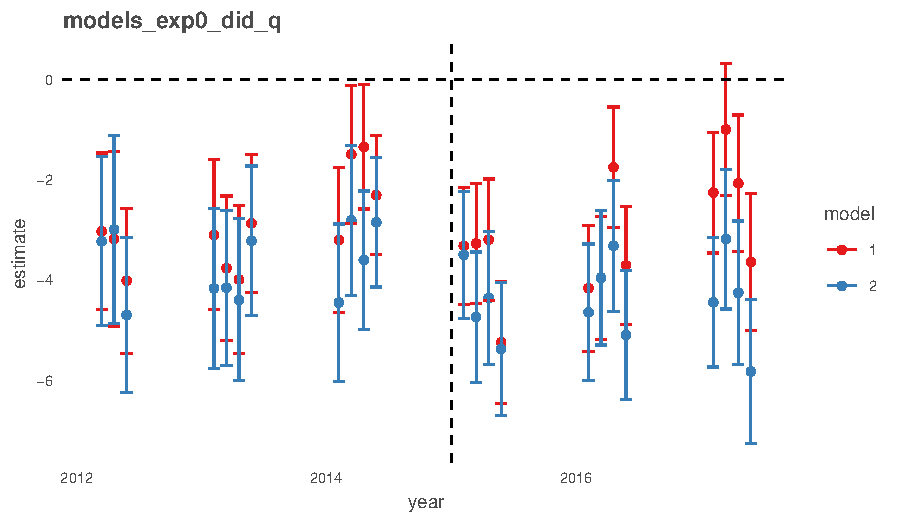
\includegraphics{C:/Users/JC/Documents/GitHub/MPA_displacement/docs/Manuscript_files/figure-latex/unnamed-chunk-20-1.pdf}
\caption{\label{fig:unnamed-chunk-20}\label{fig:q1}Interaction of quarters
and treatment. Control group is all vessels.}
\end{figure}

\begin{figure}
\centering
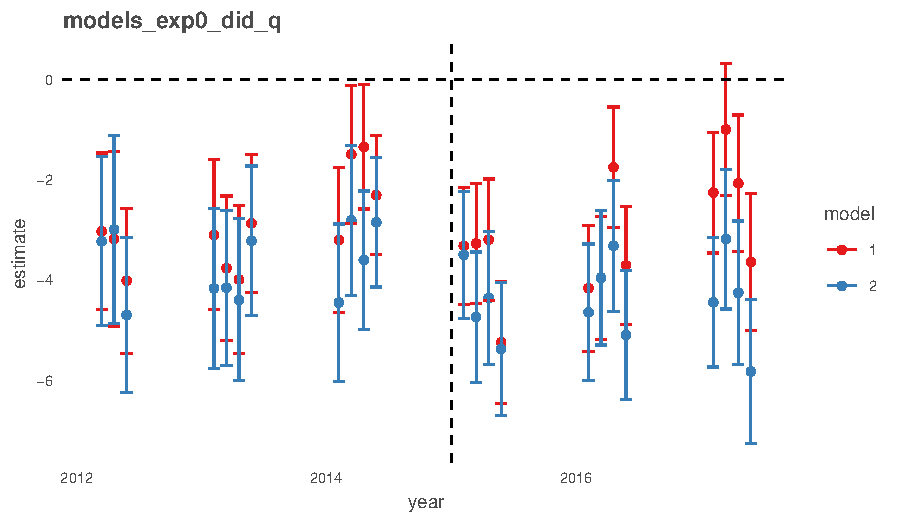
\includegraphics{C:/Users/JC/Documents/GitHub/MPA_displacement/docs/Manuscript_files/figure-latex/unnamed-chunk-21-1.pdf}
\caption{\label{fig:unnamed-chunk-21}\label{fig:q2}Interaction of quarters
and treatment. Control group is vessels from PNA.}
\end{figure}

\begin{figure}
\centering
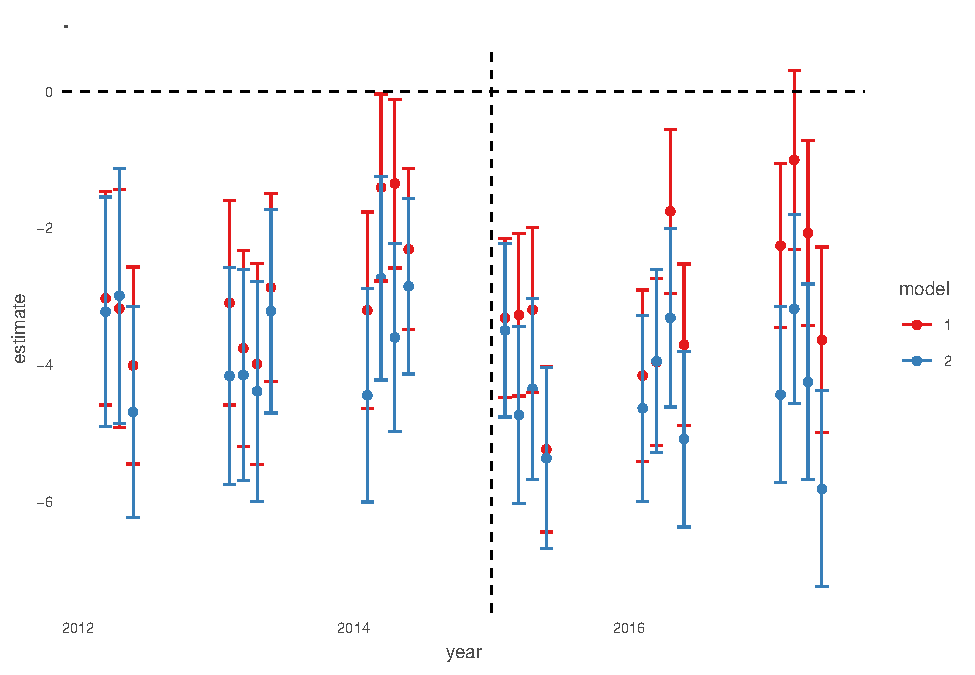
\includegraphics{C:/Users/JC/Documents/GitHub/MPA_displacement/docs/Manuscript_files/figure-latex/unnamed-chunk-22-1.pdf}
\caption{\label{fig:unnamed-chunk-22}\label{fig:q3}Interaction of quarters
and treatment. Control group excludes Chinese vessels.}
\end{figure}

\begin{figure}
\centering
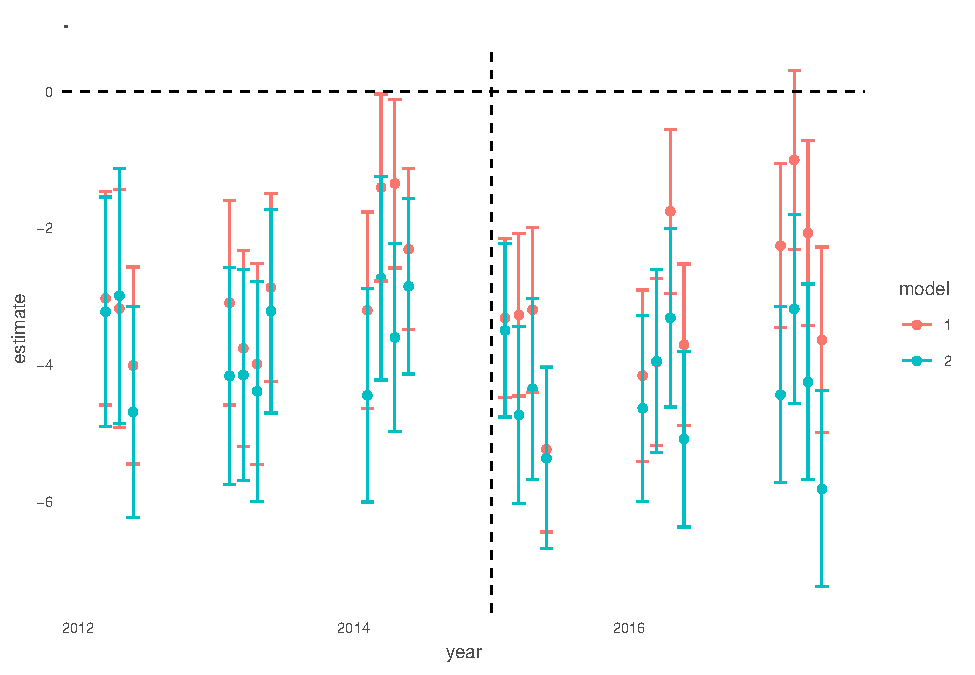
\includegraphics{C:/Users/JC/Documents/GitHub/MPA_displacement/docs/Manuscript_files/figure-latex/unnamed-chunk-23-1.pdf}
\caption{\label{fig:unnamed-chunk-23}\label{fig:q4}Interaction of quarters
and treatment. Control group is japanese vessels.}
\end{figure}

\hypertarget{year-month-did-interactions}{%
\subsubsection{Year-month DID
interactions}\label{year-month-did-interactions}}

\begin{figure}
\centering
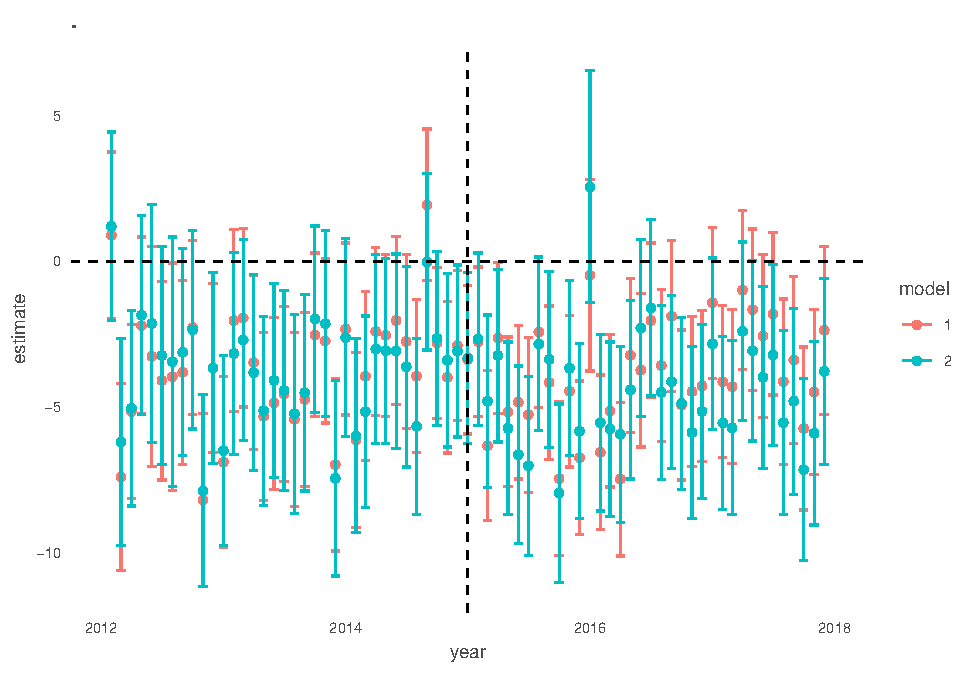
\includegraphics{C:/Users/JC/Documents/GitHub/MPA_displacement/docs/Manuscript_files/figure-latex/unnamed-chunk-24-1.pdf}
\caption{\label{fig:unnamed-chunk-24}\label{fig:ym1}Interaction of
year-month and treatment. Control group is all vessels.}
\end{figure}

\begin{figure}
\centering
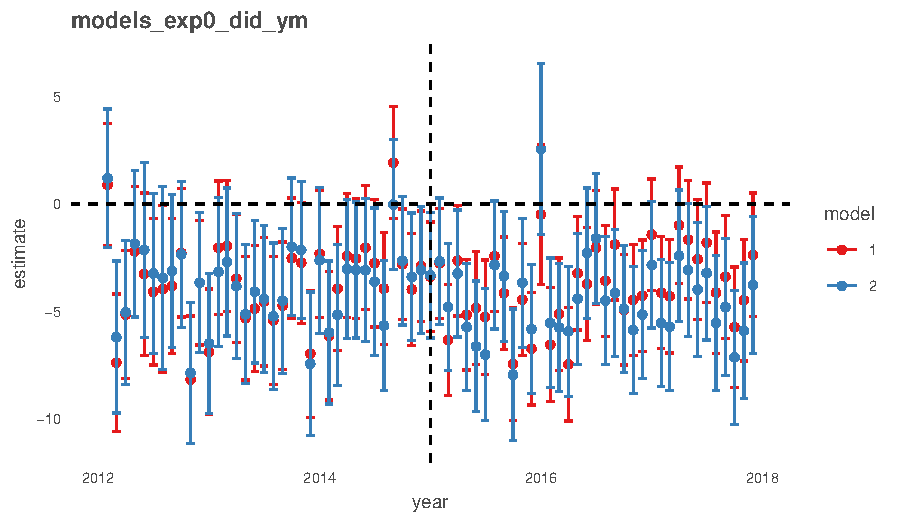
\includegraphics{C:/Users/JC/Documents/GitHub/MPA_displacement/docs/Manuscript_files/figure-latex/unnamed-chunk-25-1.pdf}
\caption{\label{fig:unnamed-chunk-25}\label{fig:ym2}Interaction of
year-month and treatment. Control group is vessels from PNA.}
\end{figure}

\begin{figure}
\centering
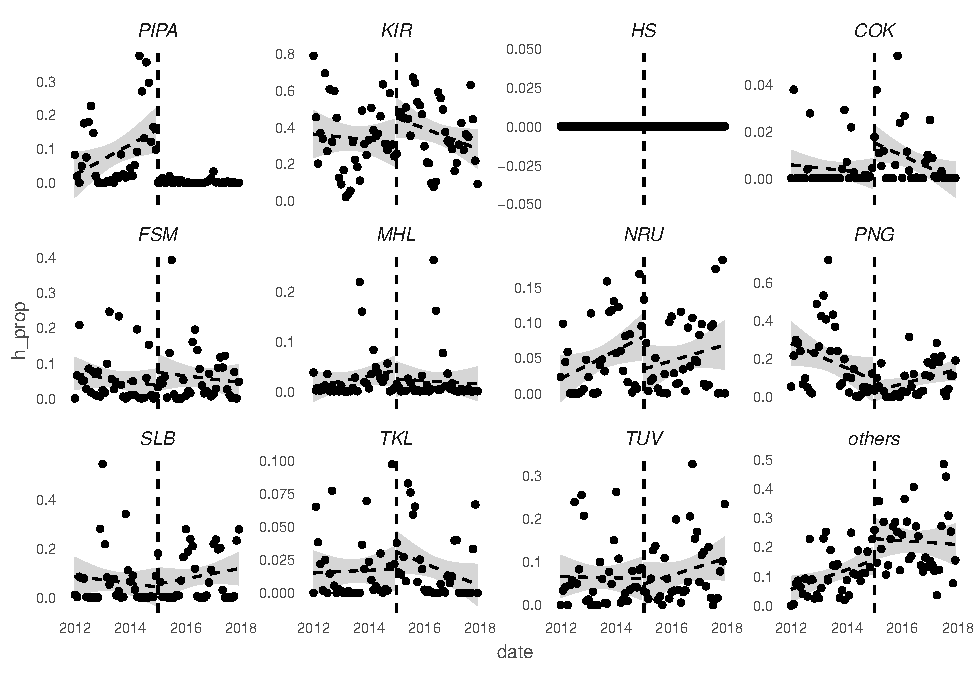
\includegraphics{C:/Users/JC/Documents/GitHub/MPA_displacement/docs/Manuscript_files/figure-latex/unnamed-chunk-26-1.pdf}
\caption{\label{fig:unnamed-chunk-26}\label{fig:ym3}Interaction of
year-month and treatment. Control group excludes Chinese vessels.}
\end{figure}

\begin{figure}
\centering
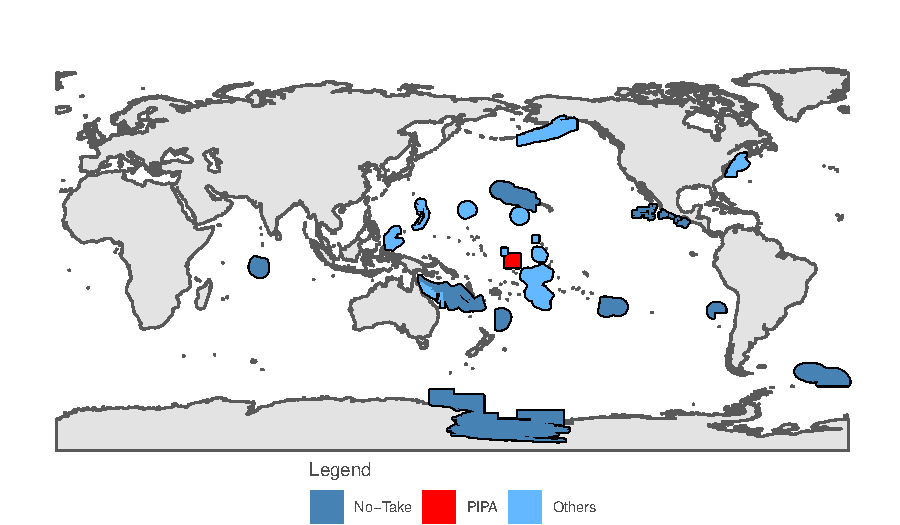
\includegraphics{C:/Users/JC/Documents/GitHub/MPA_displacement/docs/Manuscript_files/figure-latex/unnamed-chunk-27-1.pdf}
\caption{\label{fig:unnamed-chunk-27}\label{fig:ym4}Interaction of
year-month and treatment. Control group is japanese vessels.}
\end{figure}

\hypertarget{fishing-raster}{%
\subsubsection{Fishing raster}\label{fishing-raster}}

\begin{figure}
\centering
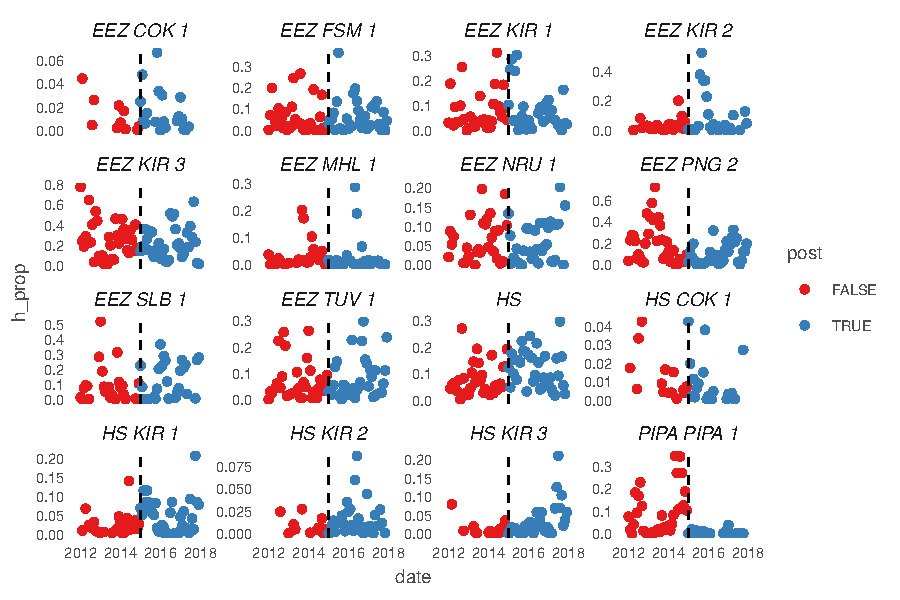
\includegraphics{C:/Users/JC/Documents/GitHub/MPA_displacement/docs/Manuscript_files/figure-latex/unnamed-chunk-28-1.pdf}
\caption{\label{fig:unnamed-chunk-28}\label{fig:fishing_raster_full}}
\end{figure}

\clearpage

\bibliography{references.bib}


\end{document}
